\section{Introduction}
\label{sec:intro}

\begin{figure}[t]
  \centering
  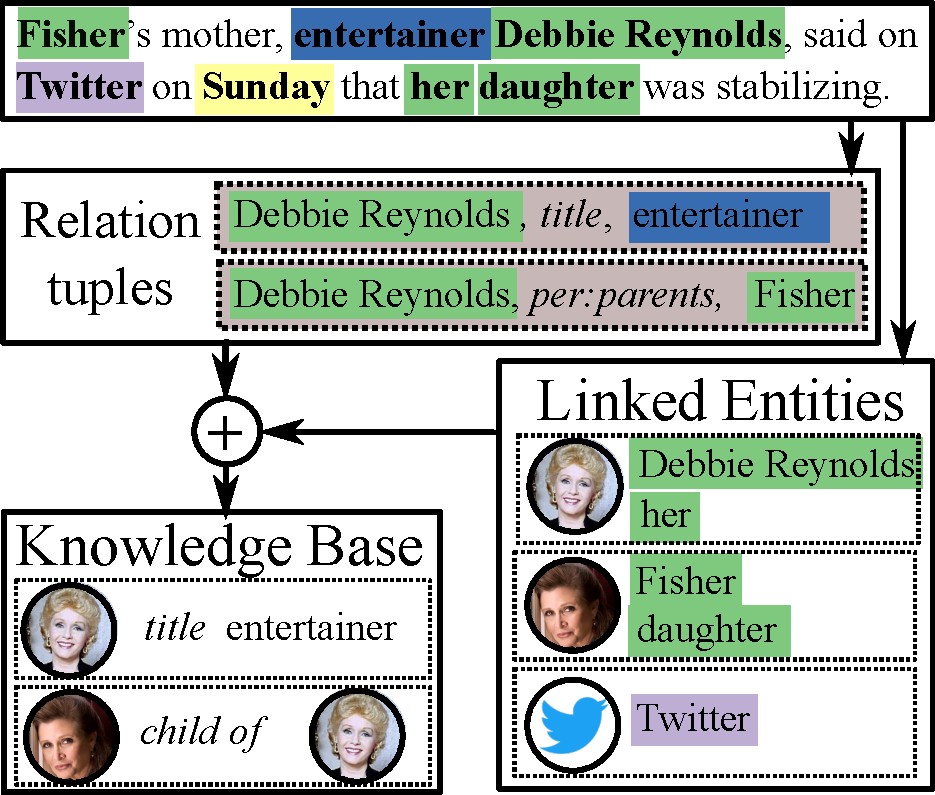
\includegraphics[width=0.9\columnwidth]{figures/entities-example.pdf}
  \caption{\label{fig:example} An example describing entities and relations in knowledge base population.}
\end{figure}

% (1 page w/ figure)
% Goal: remind the reader what information extraction is, what its relation to knowledge base population is and why it is important. Hook question.
Harnessing the wealth of information present in unstructured text online has been a long standing goal for the natural language processing community.
In particular, knowledge base population seeks to automatically construct a knowledge base consisting of relations between entities from a document corpus. % (\reffig{example}).
Knowledge bases have found many applications including question answering \citep{berant2013freebase, fader2014open,reddy2014large}, automated reasoning \citep{kalyanpur2012structured} and dialogue~\citep{han2015exploiting}.

% Evaluation @ scale poses problem. -- pooling methodology
Evaluating these systems remains a challenge as it is not economically feasible to exhaustively annotate every possible candidate relation from a sufficiently large corpus.
As a result, a pooling-based methodology is used in practice to construct datasets, similar to them methodology used in information retrieval \citep{sparck1975report, harman1993trec}.
For instance, at the annual NIST TAC KBP evaluation, all relations predicted by participating systems are pooled together, annotated and released as a dataset for researchers to develop and evaluate their systems on.
However, during development, if a new system predicts a previously unseen relation it is considered to be wrong even if it is correct.
The discrepancy between a system's true score and the score on the pooled dataset is called pooling bias and is typically assumed to be insignificant in practice~\citep{zobel1998reliable}.

% Key finding: pooling bias
The key finding of this paper contradicts this assumption and shows that the pooling bias is actually significant, and it penalizes newly developed systems by 2\% \fone{} on average (\refsec{analysis}).
Novel improvements, which typically increase scores by less than 1\% \fone{} on existing datasets, are therefore likely to be clouded by pooling bias during development.
Worse, the bias is larger for a system which predicts qualitatively different relations systematically missing from the pool.
% anti-solution
Of course, systems participating in the TAC KBP evaluation do not suffer from pooling bias, but this requires researchers to wait a year to get credible feedback on new ideas.
% TODO: I would like to add something about how ML methods are hosed, but perhaps for later?
% Chris's comment:  - Not addressed by Zobel, but I feel there is a big difference between whether this bias is a problem when used just for evaluation or also for system training (machine learning). If just for evaluation, some bias is a shame but doesn’t really badly effect things. If you are training systems assuming that your result set is the complete set of positives, then I feel that the effect of this bias is much more harmful, and this is the part that really impedes progress.

This bias is particularly counterproductive for machine learning methods as they are trained assuming the pool is the complete set of positives and are actively discouraged from predicting unseen relations and learning novel patterns.
The net effect is that researchers are discouraged from developing innovative approaches, in particular from applying machine learning models, thereby slowing progress on the task. 

%These observations may explain why rule-based systems still play such a significant role in the top submissions at TAC KBP, and why, even after 8 years, top automated systems achieve scores of only about 35\% \fone{} while human annotators score above 60\% \fone{} on the same task.

% Solution: on-demand evaluation.
Our second contribution, described in \refsec{method}, addresses this bias through a new evaluation methodology, \emph{on-demand evaluation},
which avoids pooling bias by querying crowdworkers,
while minimizing cost by leveraging previous systems' predictions when possible.
%When a researcher submits a new system's predictions to our evaluation platform,
%we carefully sample a subset of its predictions and have crowdworkers judge them.
%just enough of its predictions to guarantee an accurate estimate of scores and have crowdworkers judge them.
We then compute the new system's score based on the predictions of past systems using importance weighting.
As more systems are evaluated, the marginal cost of evaluating a new system decreases.
% Experimental results.
We then show how the on-demand evaluation methodology can be applied to knowledge base population in \refsec{application}.
Through a simulated experiment on evaluation data released through the TAC KBP 2015 Slot Validation track, we show that we are able to obtain unbiased estimates of a new systems score's while significantly reducing variance.

Finally, our third contribution is an implementation of our framework as a publicly available evaluation service at \url{https://kbpo.stanford.edu} where researchers can have their own KBP systems evaluated.
Additionally, the data collected through the evaluation process has the potential to be valuable for relation extraction, entity linking and coreference, and will also be made publicly available through the website.
each this service by evaluating three distinct systems on the 2016 TAC KBP corpus for about \$150 each (a fraction of the cost of official evaluation).
We believe the public availability of this service will speed the pace of progress in developing KBP systems.
